\section{Derivation of the approximate equations}\label{adia_improve}
Here we detail the derivation of Eq. \ref{nearly_iso_explicit} used in the 
analytical discussion of \S\ref{analytical}.  Starting with Eqs.\ \ref{lin_mass} --- \ref{lin_energy},
we set $\Gamma = 1$ and $\zeta = 0$ for the vertically isothermal limit and the fully-radially-local 
approximation, respectively.  We  eliminate
the horizontal velocity perturbations ($\delta v_x,\, \delta v_y$) to
obtain  
%we can eliminate variables 
%to obtain a pair or ordinary differential
%equations for $W,Q$ as 
\begin{subequations}\label{A1}\begin{align}
  & \ii\upsilon\delta v_z = \frac{dW}{dz} + \frac{\p\ln{\rho}}{\p z}\left(W-Q\right),\label{ode_vz} \\
  &\frac{\upsilon^2}{c_s^2}Q + \frac{\upsilon^2k_x^2}{D}W =\ii\upsilon \left(\frac{\ii
      k_x r}{D}\frac{\p\Omega^2}{\p z} -
    \frac{\p \ln{\rho}}{\p z}\right)\delta v_z - \ii\upsilon \frac{d\delta v_z}{dz},
  % \left[\frac{dW}{dz} + \frac{d\ln{\rho}}{dz}\left(W-Q\right)\right] 
  % \notag\\
  % &- \frac{d^2W}{dz^2} - \frac{d\ln{\rho}}{dz}\left(\frac{dW}{dz} -
  %   \frac{dQ}{dz}\right) - \frac{d^2\ln{\rho}}{dz^2}\left(W-Q\right),
  \label{ode_w}\\
%  &\sigma^2W - \frac{\gamma}{\Gamma}\sigma^2 Q +
%  \frac{\ii\sigma}{t_c}\left(W-\frac{Q}{\Gamma}\right) 
%  =\ii \sigma c_s^2\frac{d\ln{\rho}}{dz}\left(\frac{\gamma}{\Gamma} -
%    1\right)\delta v_z,  
  &\upsilon^2W - \gamma\upsilon^2 Q +
  \frac{\ii\upsilon}{t_c}\left(W-Q\right) 
  =\ii \upsilon c_s^2\frac{\p\ln{\rho}}{\p z}\left(\gamma -
    1\right)\delta v_z,
  % 
  % \left[\frac{dW}{dz} + \frac{d\ln{\rho}}{dz}\left(W-Q\right)\right],
  \label{ode_Q} 
\end{align}\end{subequations}
where
\begin{align}
  D \equiv \kappa^2 - \upsilon^2.
\end{align} 
%

Reduction to a single ODE requires 
$\p_zD = \p_z\kappa^2$.  At this point we could apply the 
low frequency and Keplerian approximations to set $D \rightarrow
\kappa^2 \rightarrow \OmK^2$, then $D$ is vertically constant, 
and we can obtain Eq. \ref{nearly_iso_explicit} more directly.
However, to demonstrate that the order of approximation is irrelevant,
we will retain $\p_z\kappa^2$ initially. Using 
Eq. \ref{kap2_def}---\ref{vertical_shear},  
\begin{align}\label{dkappa2}
  \frac{\p \kappa^2}{\p z} = 4 \frac{\p\Omega^2}{\p z} + r\frac{\p}{\p
    r}\frac{\p\Omega^2}{\p z} = -
  \frac{d\ln\rho}{d z}\frac{qc_s^2}{r^2} \left(
    \frac{3z^2}{r^2+z^2}-1\right) \equiv - \frac{d\ln\rho}{d z}\frac{qc_s^2}{r^2}F(r,z).
\end{align}
% For the local problem we may then write
% \begin{align}
%   \frac{dD}{dz}  = - \frac{d\ln\rho}{dz}\frac{qc_s^2}{r^2}F(z),
% \end{align}
The function $F$ increases monotonically from $F=-1$ at $z=0$ to $F\to2$
as $|z|\to\infty $, so $|F|=O(1)$. 

% In \S\ref{approx_gov} we made the replacement $D\to\OmK^2$ before
% eliminating variables to obtain a single equation for $\delta v_z$ in
% vertically isothermal disks, Eq. \ref{vertiso_gov}.  
% This procedure ignores the vertical dependence of
% $D=\kappa^2(z) - \sigma^2$. We show here that this has no serious 
% consequence for thin disks. 

%For the radially local problem, we eliminate $W$ and $Q$ from Eq. \ref{ode_w}---\ref{ode_Q} and
%Eq. \ref{lin_vz}  (with $\Gamma=1$), but now retain the vertical dependence
%of $D$ using Eq. \ref{dkappa2}, to obtain  

We  eliminate $W,\, Q$ from Eqs.\ \ref{A1}, using  Eqs. \ref{chi} and \ref{dkappa2} to obtain  
\begin{align}\label{full_ode}
  0 =& \frac{d^2\delta v_z}{dz^2} + \left[1 + \frac{\ii k_x c_s^2
      q}{Dr} - \frac{k_x^2c_s^2}{\left(k_x^2c_s^2 + \chi
        D\right)}\frac{qc_s^2F}{Dr^2}\right]\frac{d\ln\rho}{dz}\frac{d\delta
    v_z}{dz} \notag\\
  &+ \left\{\upsilon^2\left(\frac{k_x^2}{D} +
      \frac{\chi}{c_s^2}\right) + \left(\chi + \frac{\ii k_x c_s^2
        q}{Dr}\right)\frac{d^2\ln\rho}{dz^2} -
    \frac{c_s^2}{D}\left(\frac{d\ln\rho}{dz}\right)^2\left(k_x^2 -
      \frac{\ii k_x q}{r}\right)
   \left[\left(1-\chi\right) +
     \frac{\chi}{\left(k_x^2c_s^2 + \chi D\right)}\frac{qc_s^2 F}{r^2}\right] 
   \right\}\delta v_z, 
\end{align}
where we have replaced $\p/\p z$ by $d/dz$ for the
fully-radially-local treatment. Now we make the low frequency and Keplerian
approximations, setting $D\to 
\OmK^2$, to give  
\begin{align}
  &\delta v_z ^{\prime\prime} + \left[1 + \ii h q\hat{k} -
    \frac{ \hat{k}^2}{
      \left(\hat{k}^2+\chi\right)}q h^2F\right]\ln\rho^{\prime}\delta v_z^\prime +
  \left\{\left(\chi + \ii h q
      \hat{k}\right)\ln\rho^{\prime\prime} - \ln\rho^{\prime
      2}\left(\khat^2 -
      \ii h
      q\hat{k}\right)\left[1 - \chi +
      \frac{\chi}{\left(\hat{k}^2+\chi\right)}qh^2F\right]\right\}\delta v_z \notag\\&=
  -\hat{\upsilon}^2\left(\hat{k}^2+\chi\right)\delta v_z\label{adia_diso3},
\end{align} 
in terms of dimensionless variables of Eq.\ \ref{nondim}. 
Retaining terms to first order in the disk aspect ratio, $h \ll 1$, gives
\begin{align}
  0= \delta v_z ^{\prime\prime} + \left(1 + \ii h
     q\hat{k}\right)\ln\rho^{\prime}\delta v_z^\prime 
   +
   \left[\hat{\upsilon}^2\left(\hat{k}^2+\chi\right) +
     \left(  \chi + \ii h q\hat{k}\right)\ln\rho^{\prime\prime}
     - \ln\rho^{\prime
       2}\left(\khat^2 -
       \ii h
       q\hat{k}\right)\left(1 - \chi\right)\right]\delta v_z.\label{vertiso_gov_nondim}
\end{align}
Approximating the density field by Eq.\ \ref{rhoisothin} then gives 
Eq. \ref{nearly_iso_explicit}. 

We can establish a correspondence between our  Eq. \ref{nearly_iso_explicit} and
Eq. 41 in \cite{lubow93}, which describes adiabatic axisymmetric waves in
a vertically isothermal disk without vertical shear.   Accounting for the required change of variables, 
the correspondence is exact after setting $q=0$ (no vertical shear) and
$\chi=1/\gamma$ (adiabatic flow) in our Eq. \ref{nearly_iso_explicit},
and applying the approximations in our \S \ref{sec:simplified} to \citeauthor{lubow93}.    

%We comment that the simpler way
 %of obtaining Eq. \ref{vertiso_gov_nondim} is to neglect the vertical 
 %dependence of $D$ by setting $D\to\OmK^2$ in Eq. \ref{ode_w} before eliminating
 %variables in favor of $\delta v_z$.  


%Thus, a simpler route to the governing
%equation (Eq. )  

%Eq. \ref{adia_diso3} differs from Eq. \ref{vertiso_gov_nondim} by terms
%proportional to $h^2$. For a thin disk ($h\ll1$) with
%$|q|=O(1)$, as considered in this work, neglecting these terms has no
%qualitative effect on the discussion in \S\ref{analytic_relax}. 
% In deriving Eq. \ref{vertiso_gov}, the vertical dependence of
% $D=\kappa^2(z)-\sigma^2$ was ignored because the replacement
% $D\to\OmK^2$ was made before eliminating variables in favor of
% $\delta v_z$. In Appendix \ref{adia_improve} we show that making this
% replacement after eliminating variables, which involves $dD/dz$,
% introduces terms of $O(h^2)$. Since we are interested in 
% thin disks ($h\ll 1 $), e.g. protoplanetary disks where 
% $h\lesssim 0.1$ \citep{chiang10}, these terms introduce
% unnecessary complexity for the present discussion. 
      



\section{Applicability of the fully-radially-local approximation}\label{global_corr}
In the fully-radially-local approximation, background radial
gradients are ignored except where it appears
implicitly in the expression for the vertical shear rate $\p_z\Omega$
(via Eq. \ref{vertical_shear}).  This is done by neglecting the terms proportional to $\zeta$
in Eq. \ref{lin_mass}, \ref{lin_vx} and \ref{lin_energy}, i.e. setting 
$\zeta=0$. (Nomially $\zeta=1$, which is used in our numerical study.) 


For a power-law disk, the neglected radial gradients   
are $O(r^{-1})$, and they appear in comparison with terms of
$O(k_x)$. The neglected terms therefore have a relative magnitude of
$O(h/\khat)$, which is small for thin disks ($h\ll1$) 
and/or small radial wavelengths ($\khat\gg 1$).  We show in the
following sections that the fully-radially-local approximation only 
becomes invalid in the adiabatic limit, which is not the relevant
regime for the VSI. 

We comment that this approximtaion is equivalent to 
that adopted in the vertically global shearing box formalism
\citepalias[VGSB,][]{mcnally14}, which is an 
extension of the standard shearing box \citep{goldreich65} to
background shear flows that are height dependent.

%However, background radial gradient terms 
%are ignored elsewhere in the VGSB (which is done by setting
%$\zeta=0$).         
   
% \begin{align}
%   \ii \sigma W  &=c _s^2(r_0, z)\left( \left.\frac{\p\ln\rho}{\p
%       z}\right|_0 \delta v_z + \frac{\gamma}{\Gamma} \frac{d\delta
%     v_z}{dz}\right) + \left[\ii k_xc_s^2(r_0,z)
%   \frac{\gamma}{\Gamma} + \zeta\left.\frac{1}{\rho}\frac{\p P}{\p
%       r}\right|_0\right]\delta v_x  +
% \frac{1}{t_c}\left(W-\frac{Q}{\Gamma}\right),\label{gcorr_terms1}\\
% \ii \sigma Q &= c_s^2(r_0,z)\left(\ii k_x + \zeta
%   \left.\frac{\p\ln{\rho}}{\p r}\right|_0\right)\delta v_x + c _s^2(r_0, z)\left( \left.\frac{\p\ln\rho}{\p
%       z}\right|_0 \delta v_z + \frac{d\delta
%     v_z}{dz}\right),\label{gcorr_terms2} \\
% \ii \sigma \delta v_x & = \ii k_x W  -
% \zeta\frac{1}{c_s^2(r_0,z)}\left.\frac{1}{\rho}\frac{\p P}{\p
%   r}\right|_0Q - 2\Omega(r_0,z)\delta v_y,\label{gcorr_terms3}
% \end{align}
% where subscript $0$ denotes evaluation at $r=r_0$. We recall terms
% proportional to $\zeta$ are associated with the background density
% and pressure radial structures, and nominally $\zeta=1$.   

\subsection{Spurious growth of adiabatic perturbations when
  $\zeta=0$}\label{analytic_adia}  
A limitation of the reduced model described in Appendix
\ref{adia_improve}, \S\ref{sec:simplified} and used in \S\ref{analytical}, is that it
cannot be employed for adiabatic flow when there is vertical shear, even
if $h/\khat\ll1$.  We explain this by setting  $\beta\to\infty$ and hence $\chi = 1/\gamma$ in 
Eq. \ref{vertiso_gov_nondim} % (which itself is obtained by setting
% $\zeta=0$ in Eq. \ref{lin_mass}---\ref{lin_energy})
to give 
\begin{align}
  0 =\dd v_z^{\prime\prime} + \left(1 + \ii h q
    \hat{k}\right)\left(\ln\rho^{\prime}\delta v_z\right)^\prime
  +\left\{\hat{\upsilon}^2\left(\frac{1}{\gamma}+\hat{k}^2\right) 
    -\left(\frac{\gamma-1}{\gamma}\right)\left[\ln\rho^{\prime\prime}+\hat{k}^2\left(1-\frac{\ii h  
          q}{\hat{k}}\right)\ln\rho^{\prime 2}\right]\right\}\delta v_z.\label{adia_iso3}
\end{align}
We multiply Eq. \ref{adia_iso3} by $\rho\delta v_z^*$ and
integrate vertically, assume boundary terms vanish when integrating by
parts, to obtain
\begin{align}
  \hat{\upsilon}^2\left(\frac{1}{\gamma} +
    \hat{k}^2\right)\int_{\zhat_1}^{\zhat_2}\rho|\delta
  v_z|^2 d\zhat 
  =&  \left(\frac{\gamma-1}{\gamma}\right)
  \int_{\zhat_1}^{\zhat_2}\rho|\delta v_z^\prime|^2 d\zhat
  +\frac{1}{\gamma}\int_{\zhat_1}^{\zhat_2}\frac{1}{\rho}|(\rho\delta
  v_z)^\prime|^2 d\zhat\notag\\
&+
  \left(\frac{\gamma-1}{\gamma}\right)\hat{k}^2\left(1-\frac{\ii h
      q}{\hat{k}}\right) \int_{\zhat_1}^{\zhat_2}\rho\ln\rho^{\prime
    2}|\delta v_z|^2 d\zhat
+ \ii h q \hat{k}
  \int_{\zhat_1}^{\zhat_2}\ln\rho^\prime(\rho\delta v_z^*)^\prime
  \delta v_z d\zhat.\label{adia_integral}
\end{align}
% When $q\equiv0$, all the terms on the right-hand-side (RHS) are real. Then
% $\hat{\upsilon}^2$ is real, and  $\hat{\upsilon}^2>0$ if $\gamma>1$. As
% expected, a sub-adiabatically stratified disk is stable in the absence
% of vertical shear. 
In the presence of vertical shear $q\neq0$, Eq. \ref{adia_integral}
suggests $\hat{\upsilon}^2$ is complex for real $\khat$, which implies the
possibility of instability, regardless of the value of
$|\gamma-1|$. This is contradicts the second Solberg-Hoiland criterion 
(Eq. \ref{solberg2}), which imply instability for adiabatic
perturbations in a thin, vertically isothermal disk would require 
$|\gamma-1|\ll1$. 
%also need real freq^2 in adia limit 
This is because we have retained the global radial temperature 
gradient to obtain vertical shear, 
but have ignored it elsewhere in the linear problem (as well as the
background radial density gradient). Nevertheless, we demonstrate below
that this inconsistency is unimportant for the VSI, which occurs 
for $\beta\ll1$.   %and small scale

\subsection{Effect of global radial gradients}
In  Fig. \ref{gcorr_compare}, we plot the effect of the global radial gradient terms
proportional to $\zeta$ in Eq. \ref{lin_mass}---\ref{lin_energy}
by calculating the
fundamental VSI growth rates using three approaches. We compute growth rates from the dispersion
relation Eq. \ref{relax_disp}, which assumes $\zeta=0$;  from
Eq. \ref{lin_mass}---\ref{lin_energy} with $\zeta=0$; and from
Eq. \ref{lin_mass}---\ref{lin_energy}  with $\zeta=1$.   

All three methods give similar behavior, and growth rates are in close
agreement for $\beta\lesssim 1$. Differences arise for 
$\beta\gtrsim1$, and as $\beta\to\infty$ the fully-radially-local
approximation, where $\zeta=0$, gives a
(spurious) growth rate as expected from the discussion
above. Inclusion of the global radial gradient terms results in the
expected behavior  ($\sigma\to0$ as $\beta\to\infty$). Despite this
caveat, Fig. \ref{gcorr_compare} shows that provided we consider 
$\beta\lesssim O(1)$, then setting $\zeta=0$ does not affect the VSI
significantly.  
  
\begin{figure}
  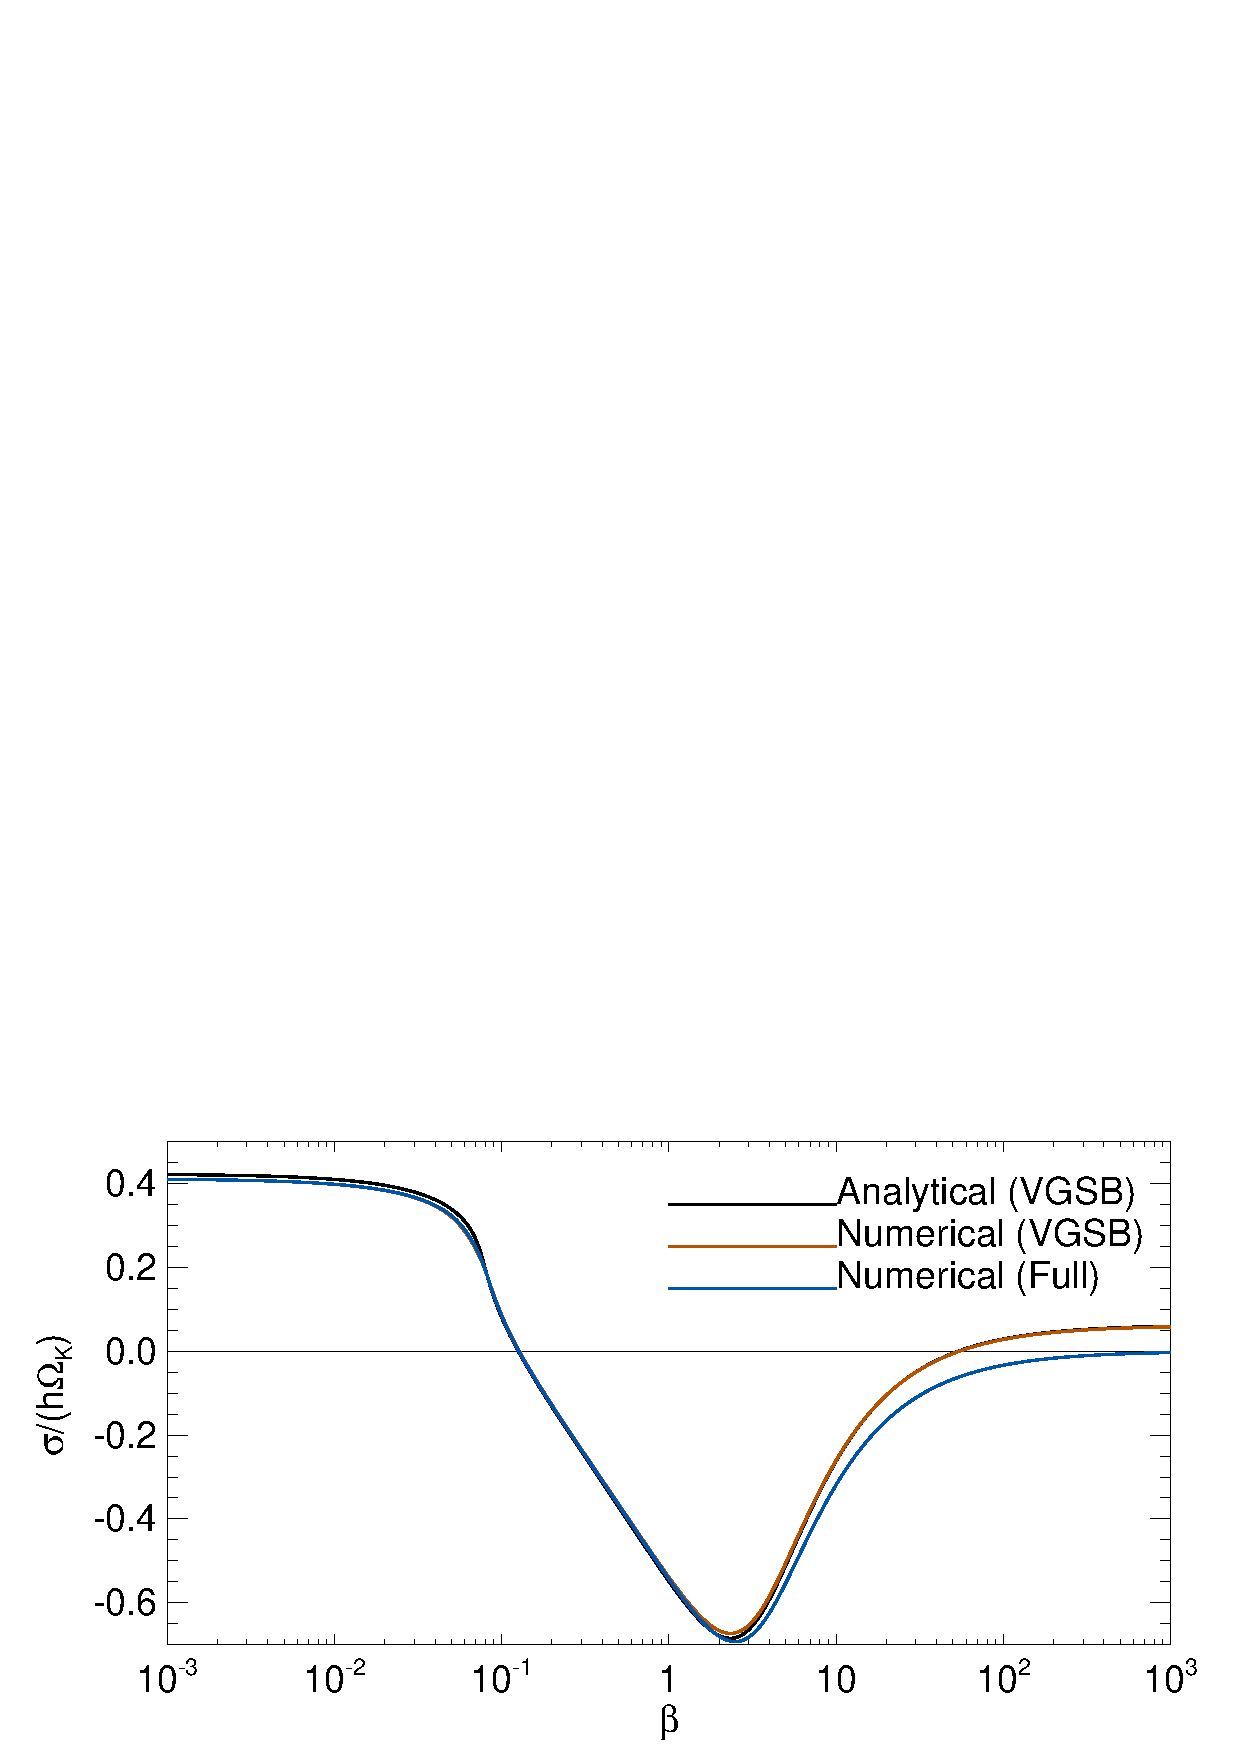
\includegraphics[width=\linewidth,clip=true,trim=0cm 0.0cm 0cm
  0cm]{figures/gcorr_compare} 
  \caption{Growth rate of the fundamental VSI mode as a function of
    the thermal relaxation time $\beta$. The `Analytical ($\zeta=0$)' curve
    is calculated from the dispersion relation Eq. \ref{relax_disp}. 
    The `Numerical ($\zeta=0$)' curve is obtained from the numerical
    solution to Eq. \ref{lin_mass}---\ref{lin_energy} with
    $\zeta=0$,  which 
    neglects explicit dependencies on the radial disk structure.  
    The `Numerical
    ($\zeta=1$)' curve is obtained from Eq. \ref{lin_mass}---\ref{lin_energy} with
    $\zeta=1$, which accounts for the radial disk structure self-consistently.   
    The disk parameters are $(\gamma, \Gamma)=(1.4, 1.011)$ and
    $(p,q,h)=(-1.5,-1,0.05)$. The perturbation 
    wavenumber is $\khat=30$. 
    \label{gcorr_compare}}  
\end{figure}










\section{Linear problem in the isothermal limit}\label{iso_discuss}  
Here we summarize selected results for isothermal
perturbations ($\beta\equiv 0$) in vertically isothermal disks 
($\Gamma=1$) in the fully-radially local approximation
($\zeta=0$). In this case Eq. \ref{ode_Q}
becomes    
\begin{align} 
  Q = W 
\end{align}
(i.e. $\delta P = c_s^2\delta \rho$)% , and so $  \ii\hat{\upsilon}c_s\delta v_z = W^\prime $
% from Eq. \ref{lin_vz}
. For isothermal perturbations it is 
simpler to work with an equation for $W$ by substituting $Q=W$ into
Eq. \ref{ode_w} and using Eq. \ref{ode_vz} to eliminate $\delta v_z$. 
In this case, we shall not yet make the low frequency
approximation, but first make the  Keplerian approximation. We
obtain, in terms of dimensionless variables, 
\begin{align}
  0 = W^{\prime\prime} + \left[\ln\rho^\prime - \frac{\ii h q \hat{k} f(\zhat)
      }{1-\hat{\upsilon}^2} \right]W^\prime +
  \hat{\upsilon}^2\left(1+\frac{\hat{k}^2}{1-\hat{\upsilon}^2}\right)W,\label{iso_ode0} 
\end{align}
where for discussion purposes we have defined $f(\zhat)$ such that
\begin{align}\label{fz_shear}
  \frac{d\Omega^2}{d\hat{z}} = h^2q f(\hat{z})\OmK^2.
\end{align}
By comparing Eq. \ref{fz_shear} with Eq. \ref{vertical_shear_ex}, we
see that $f(\zhat)= 
\zhat\left(1+h^2\zhat^2\right)^{-3/2}$. More generally, though,
$f$ may be regarded as a representation of the vertical
shear profile. Physically, we expect there is a maximum value of 
$|d\Omega/dz|$, the existence of which should limit the growth rate of
the VSI,  as remarked in \S\ref{vshear_def}. We explicitly demonstrate
this below.     

\subsection{Maximum growth rate  in the low-frequency limit}
Here we consider the low-frequency limit $|\hat{\upsilon}|\ll 1$ and 
show that the growth rate is limited by the maximum vertical
shear rate in the domain. 
%In the low-frequency limit we assume $|\hat{\upsilon}|\ll 1$ and
We approximate Eq. \ref{iso_ode0} as 
\begin{align}
  0 = W^{\prime\prime} + \left[\ln\rho^\prime - \ii h q \hat{k}
    f(\zhat)\right]W^\prime +
  \hat{\upsilon}^2\left(1+\hat{k}^2\right)W. \label{iso_ode1}
\end{align}
%\subsubsection{Necessity of vertical shear for
%  instability}\label{integral_relation} 
%We can establish a necessary condition for instability 
We multiply Eq. \ref{iso_ode1} by $\rho W^*$ and integrate vertically from
$\zhat=\zhat_1$ to $z=\zhat_2$. We neglect boundary 
terms when integrating by parts, by assuming $W$ or
$W^\prime$ vanishes at the boundaries, or that the boundaries are 
sufficiently far away so that the boundary terms are negligible because of the
decaying background density with increasing height. Then,
\begin{align}
  \hat{\upsilon}^2\left(1+\hat{k}^2\right)\int_{\zhat_1}^{\zhat_2}\rho|W|^2d\zhat
  =\int_{\zhat_1}^{\zhat_2}\rho|W^\prime|^2d\zhat 
  +\ii h q \hat{k}\int_{\zhat_1}^{\zhat_2}\rho f(\zhat) W^*W^\prime d\zhat.\label{integral_relation1}
\end{align}
It follows that for instability ($\imag\hat{\upsilon}>0$), it is necessary to
have $q\neq0$ or more generally $d\Omega/dz\neq 0$, i.e. there must
be vertical shear. 
%A similar conclusion can be reached in the
%equivalent linear problem in global cylindrical disk geometry.  
%\subsubsection{Maximum growth rate}\label{max_growth1}

The real and imaginary parts of 
Eq. \ref{integral_relation1} are
\begin{align}
  \left(\hat{\omega}^2-\hat{\sigma}^2\right)\left(1+\hat{k}^2\right) 
  \int_{\zhat_1}^{\zhat_2}\rho|W|^2d\hat{z} -
  \int_{\zhat_1}^{\zhat_2}\rho|W^\prime|^2d\hat{z}
  \notag
  =\real\left[\ii
    h\hat{k}q \int_{\zhat_1}^{\zhat_2}\rho
    f(\hat{z}) W^*W^\prime d\zhat\right], \\
   2\hat{\omega}\hat{\sigma}\left(1+\hat{k}^2\right)
  \int_{\zhat_1}^{\zhat_2}\rho|W|^2d\hat{z}
  =\imag\left[\ii
    h\hat{k}q \int_{\zhat_1}^{\zhat_2}\rho
    f(\hat{z}) W^*W^\prime d\hat{z}\right],
\end{align}
where we recall $\hat{\omega} = \real \hat{\upsilon}$ and
$\hat{\sigma}=\imag\hat{\upsilon}$. 
Adding the square of these equations give
\begin{align}
  \left[|\hat{\upsilon}|^2\left(1+\hat{k}^2\right)
    \int_{\zhat_1}^{\zhat_2}\rho|W|^2d\hat{z} -
    \int_{\zhat_1}^{\zhat_2}\rho\left|W^\prime \right|^2d\hat{z}\right]^2
  +4\hat{\sigma}^2\left(1+\hat{k}^2\right) 
  \int_{\zhat_1}^{\zhat_2}\rho
  |W|^2d\hat{z}\int_{\zhat_1}^{\zhat_2}\rho\left|W^\prime \right|^2d\hat{z}
  =\left|\ii
    h\hat{k}q\int_{\zhat_1}^{\zhat_2}\rho
    f(\hat{z}) W^*W^\prime d\hat{z}\right|^2.
\end{align}
It is clear that
\begin{align}\label{sigma_finite_domain} 
  4\hat{\sigma}^2\left(1+\hat{k}^2\right) 
  \int_{\zhat_1}^{\zhat_2}\rho
  |W|^2d\hat{z}\int_{\zhat_1}^{\zhat_2}\rho\left|W^\prime
  \right|^2d\hat{z} 
  \leq\left|
    h\hat{k}q\int_{\zhat_1}^{\zhat_2}\rho
    f(\hat{z}) W^*W^\prime d\hat{z}\right|^2.
\end{align}
On the left hand side of this inequality, we apply the Cauchy-Schwarz
inequality to obtain
\begin{align}
  \left( \int_{\zhat_1}^{\zhat_2}\rho
    |W|\left|W^\prime \right|d\hat{z}\right)^2\leq
  \int_{\zhat_1}^{\zhat_2}\rho 
  |W|^2d\hat{z}\int_{\zhat_1}^{\zhat_2}\rho\left|W^\prime \right|^2d\hat{z}.
\end{align}
On the right hand side of Eq. \ref{sigma_finite_domain} we have
\begin{align}
  \left|\int_{\zhat_1}^{\zhat_2}\rho
    f(\hat{z}) W^*W^\prime d\hat{z}\right|\leq \int_{\zhat_1}^{\zhat_2}\rho
  \left|f(\hat{z})W^*W^\prime \right|d\hat{z}
  \leq
  \mathrm{max}\left(|f|\right)\int_{\zhat_1}^{\zhat_2}\rho
  |W|\left|W^\prime \right|d\hat{z},
\end{align}
where $\mathrm{max}(|f|)$ is the maximum value of $|f|$ in
$\zhat\in[\zhat_1,\zhat_2]$. Inserting these inequalities into
Eq. \ref{sigma_finite_domain} gives
\begin{align}\label{max_growth}
  |\hat{\sigma}|\leq
  \frac{h |\hat{k} q|}{2\sqrt{1+\hat{k}^2}}\mathrm{max}(|f|) < \frac{h |q|}{2}\mathrm{max}(|f|) . 
\end{align}
%Recalling that $f$ represents vertical shear (Eq. \ref{fz_shear}), 
It
follows that the maximum possible growth rate of unstable modes,
satisfying the above boundary conditions, is limited by the maximum
vertical shear rate in the domain considered,
\begin{align}
  |\sigma| < \mathrm{max} \left|r\frac{d\Omega}{dz}\right|, 
\end{align}
as expected on physical grounds. %A similar conclusion can be reached in the
%equivalent linear problem in global cylindrical disk geometry.  

In practice, one might consider a vertical domain of a few scale 
heights in a thin disk with $|q|=O(1)$. In this case, $|h\zhat|\ll1$ and  
$f\simeq \zhat$, so that $\mathrm{max}|f| = O(1)$, implying a
maximum growth rate $O(h \OmK)$, consistent with numerical
results. 

\subsection{Explicit solutions in the thin-disk limit}\label{iso_explicit}
Here we assume a thin disk ($h\ll1$) so that $\ln\rho\simeq
-\zhat^2/2$ and $f(\zhat)\simeq \zhat$. However, we do not assume 
low frequency from the onset. Then Eq. \ref{iso_ode0} becomes 
\begin{align}\label{iso_ode3}
  W^{\prime\prime} - \left(1 + \frac{\ii qh \hat{k}}{1-\hat{\upsilon}^2}\right)\hat{z}W^\prime  +
  \hat{\upsilon}^2\left(1+\frac{\hat{k}^2}{1-\hat{\upsilon}^2}\right)W = 0.
\end{align}
We remark that taking the low frequency limit and considering
$\hat{k}^2\gg 1$, Eq. \ref{iso_ode3} becomes equivalent to Eq. 39 in
\citetalias{nelson13} or Eq. 28 in \citetalias{barker15}, although we have taken a
different route.    
 
% To complete the problem we must specify boundary conditions. The 
% maximum vertical domain size should be limited by the thin
% disk and low-frequency approximations (i.e. $z\lesssim r$).     
%It is, however, common to take $\mathrm{max}|z|\to\infty$ and 

We seek power series solutions to Eq. \ref{iso_ode3}, 
\begin{align}
  W(\zhat) = \sum_{l=0}^\infty a_l\zhat^l. 
\end{align}
Then the coefficients $a_l$ are given by the recurrence relation
\begin{align}
  (l+2)(l+1)a_{l+2} +
  \left[\hat{\upsilon}^2\left(1+\frac{\khat^2}{1-\hat{\upsilon}^2}\right)
    - l\left(1+\frac{\ii h q
        \hat{k}}{1-\hat{\upsilon}^2}\right)\right] a_l = 0. 
\end{align}
We demand the series to terminate  at $l=L$, i.e. a polynomial of
order $L$, so that the vertical kinetic energy density remain bounded as 
$|\zhat|\to\infty$.  Then the eigenfrequency $\hat{\upsilon}$ is given via 
\begin{align}
\hat{\upsilon}^4 - \left(L+1+\khat^2\right)\hat{\upsilon}^2 + L\left(1 +
  \ii h q \khat\right) = 0. \label{simple_growth}
\end{align}

Note that we have applied a regularity condition at infinity, since
the vertically isothermal disk has no surface. If vertical boundaries
are imposed at finite height, as done in numerical calculations, then
the above solution needs to be modified to match the desired boundary
conditions. This enables the `surface modes' seen in numerical
calculations \citepalias{barker15}. 

\subsubsection{Stability without vertical shear}\label{stable_novshear}
In the absence of vertical shear $q=0$, Eq. \ref{simple_growth} can be
written as \begin{align}
  \hat{\upsilon}^2\khat^2 =
  \left(L-\hat{\upsilon}^2\right)\left(1-\hat{\upsilon}^2\right), \label{iso_disp_full}
\end{align}
which is just the dispersion relation for axisymmetric isothermal waves in a
vertically isothermal disk (e.g. \citealt{okazaki87}; \citealt{takeuchi98}; \citealt{tanaka02}; 
\citealt{zhang06}; \citealt{ogilvie13}; \citealt{barker14}; \citetalias{barker15}). In 
this case the solutions are Hermite polynomials, $W\propto
\He_L(\zhat)$.  The eigenfrequency $\hat{\upsilon} = \hat{\omega}$ is real and the disk
is stable. The low frequency branch of Eq. \ref{iso_disp_full} are 
inertial waves \citep{balbus03}. For 
$|\hat{\omega}|\ll 1$ and $L\geq 1$ the dispersion relation is
$\hat{\omega}^2\khat^2 = L$, or $\hat{\omega}\propto \khat^{-1}$ for
fixed $L$. This inverse relation has been qualitatively
observed in numerical simulations of \cite{stoll14}. 
Note that $L=M+1$, where $M\geq 0$ is the mode number used for analytical
discussion (\S\ref{analytical}) based on the reduced equation for
$\delta v_z$, rather than for $W$ as considered here. 
%Note that for
%analytical discussions (\S\ref{analytical}) we work with an equation
%for $\delta v_z$ so that $L=M+1$.  

\subsubsection{Instability with vertical shear}
The VSI corresponds to unstable inertial waves. This
is readily obtained for large $\khat^2$ by balancing
the last two terms of Eq. \ref{simple_growth} to give the low
frequency branch. Then 
\begin{align}
  \hat{\upsilon}^2 \simeq L\left(\frac{1+\ii q h
       \hat{k}}{L+1+\hat{k}^2}\right), \label{simple_growth2}
\end{align}
which is equivalent to Eq. 34 of \citetalias{barker15} in the limit
$\khat^2\gg L$. This signifies instability for
$L\geq1$ since we can choose the sign 
of the square root to make $\hat{\sigma} = \imag\hat{\upsilon}>0$.  These
are the low frequency unstable modes seen in
Fig. \ref{compare_modes_iso_kx10} and
Fig. \ref{compare_modes_iso_kx30}, for which $\sigma\propto|\omega|$.  

\section{Analytic dispersion relation
with thermal relaxation}
\subsection{Coefficients}\label{relax_coeff}
The coefficients of the dispersion relation Eq.\ \ref{relax_disp} are:
\begin{subequations}\label{coeffs}\begin{align}
  &c_0 = M(M+1)A^2,\\
  &c_1 = \ii\beta\left\{\left(1-\gamma\right)\left[1 +
      \khat^2\left(1+2M\right)^2 - 4 \ii h q\khat M (M+1)\right] 
    - 2A^2\gamma M (M+1)\right\},\\
  &c_2 = \left(\khat^2 + 1\right)A + \beta^2\left\{(1-\gamma)\left[1
      + \gamma \khat^2(1+2M)^2 - 4\ii h q \khat \gamma M(M+1)
    \right]
    -\gamma^2 A^2 M(M+1)
  \right\},\\
  &c_3 = \beta\left\{h q \khat + \gamma \left[\ii + h q
      k \left(1+2\khat^2\right)\right] - 3\ii - 2\ii
    \khat^2\right\},\\
  &c_4 =
  \beta^2\left(1+\gamma\khat^2\right)\left[\gamma\left(1-\ii h q
    \khat\right)-2\right] - \left(1+\khat^2\right)^2,\\
&c_5 = 2\ii\beta\left(1+\khat^2\right)\left(1+\gamma\khat^2\right),\\
&c_6 = \beta^2\left(1+\gamma\khat^2\right)^2.
\end{align}\end{subequations}

\subsection{Finding marginal stability}\label{disp_neut_limit}
To investigate marginal stability we set $\hat{\sigma} = 0$ so the
frequency, $\hat{\upsilon}=\hat{\omega}_c$, is real; and $\beta =
\beta_c$,  the cooling time for marginal stability. 
We take the short radial wavelength limit, $\khat^2\gg 1$, of the
coefficients in Eq.\ \ref{coeffs}. We consider $M \lesssim O(1)$ and
assume $\beta_c \ll \khat$.  The real and 
imaginary parts of Eq. \ref{relax_disp} then give relations for $\hat{\omega}_c$ and $\beta_c$ as 
\begin{align}
  0 =&M(M+1)(1-h^2 q^2 \khat^2) + 4\beta_c h q M(M+1)\left(\hat{\omega}_c\khat\right) 
 +\left[1 +
    \gamma\beta_c^2\left(1-\gamma\right)(1+2M)^2\right]\left(\hat{\omega}_c\khat\right)^2 \label{relax_cond1} \\
 &+ 2h q \gamma\beta_c \left(\hat{\omega}_c\khat\right)^3 -  \left(\hat{\omega}_c\khat\right)^4 
  + \beta_c^2\gamma^2\hat{\omega}_c^2
  \left(\hat{\omega}_c\khat\right)^4, \notag \\
   0=& 2h q M (M+1)\khat +
   \beta_c(1-\gamma)(1+2M)^2\khat\left(\hat{\omega}_c\khat\right) 
   + h q \khat \left(\hat{\omega}_c\khat\right)^2 -
   2\beta_c\hat{\omega}_c\left(\hat{\omega}_c\khat\right)^2
   - h q
   \gamma^2\beta_c^2\hat{\omega}_c\left(\hat{\omega}_c\khat\right)^3 \label{relax_cond2} \\
   &+
   2\beta_c\gamma\hat{\omega}_c\left(\hat{\omega}_c\khat\right)^4 \notag. 
\end{align}
We recall that in the low frequency and thin-disk approximations, $h,
|\hat{\omega}_c| \ll 1$. We note that $|q|=O(1)$ and 
$\gamma>1$ but is $O(1)$. We assume $|\hat{\omega_c}\khat|=O(1)$,
since for inertial waves $|\hat{\omega}\khat|\simeq \sqrt{1 + M}$. Finally, we further assume 
$\beta_c \ll 1$, to be justified \emph{a posteriori}, to give 
Eq. \ref{relax_cond_simp1}---\ref{relax_cond_simp2}.   

\subsection{Maximum critical cooling time}\label{max_cool}   
Here we show that, under appropriate conditions, the longest critical 
cooling time is that for the $M=0$ or fundamental mode. This allows
us to focus on the fundamental mode to obtain an overall cooling
requirement for the VSI.      

Consider the simplified dispersion relations for marginal stability,
Eq. \ref{relax_cond_simp1}---\ref{relax_cond_simp2}. We write 
$X= \hat{\omega}\khat$, $\theta = (hq\khat)^2$ and  
treat $M$ as a continuous variable. We find from
Eq. \ref{relax_cond_simp1} that  
%\begin{align}
%  &x^4  = x^2 + M(M+1)(1-\theta), \label{simp1}\\
%  &x^2  = \frac{\gamma-1}{h q}\beta_c (1+2M)^2x - 2M(M+1)\label{simp2},
%\end{align}
%where and
\begin{align}
  2 X \frac{d X}{dM} = \frac{X^2(1-\theta)(2M+1)}{X^2 +
  2M(M+1)(1-\theta)}, 
\end{align}
and from Eq. \ref{relax_cond_simp2} that
\begin{align}
  2X\frac{dX}{dM} = \left[X^2 +
  2M(M+1)\right]\left(\frac{d\ln{\beta_c}}{dM} + \frac{4}{2M+1} +
  \frac{d\ln{X}}{dM}\right) - 2(2M+1). 
\end{align}
We eliminate $dX/dM$, making use of Eq. \ref{relax_cond_simp1} in the process, to obtain 
\begin{align}
  (2M+1)\frac{d\ln{\beta_c}}{dM} %= \frac{\mathcal{N}}{\mathcal{D}}, 
  = -\frac{(1-\theta)M(M+1)\left[ 2(2M+1)^2 + 12X^2\right]
  + (3+\theta)X^2}{2 \left[X^2 +
  2M(M+1)(1-\theta)\right]\left[X^2 + 2M(M+1)\right]}.  
\end{align}
%where the denominator $\mathcal{D}$ is
%\begin{align}
%\mathcal{D} = 2 \left[X^2 +
 % 2M(M+1)(1-\theta)\right]\left[X^2 + 2M(M+1)\right]>0, 
%\end{align}
%and the numerator $\mathcal{N}$ is 
%\begin{align}
 % \mathcal{N} = -(1-\theta)\left[ 2M(M+1)(2M+1)^2 + 12X^2M(M+1)\right]
 % - (3+\theta)X^2 < 0.
%\end{align}
Hence,
\begin{align}\label{dbeta_dm}
  \frac{d\beta_c}{dM}<0, 
\end{align}
for all $M\geq 0$ if $\theta\leq 1$, which imply 
$\mathrm{max}(\beta_c)$ occurs at $M=0$. This result may also be
obtained by explicitly solving 
Eq. \ref{relax_cond_simp1}---\ref{relax_cond_simp2} with $\theta$
treated as a small parameter. For fixed $\khat$ the 
condition $\theta\leq 1$ can be satisfied in sufficiently thin disks.
All such modes are stabilized if
$\beta>\beta_c(M=0)\equiv\beta_\mathrm{crit}$. 

This result highlights the importance of the fundamental mode  
--- it is the most difficult mode to stabilize with finite
cooling. Furthermore, for $M=0$ we may obtain the expression  
for $\beta_\mathrm{crit}$ from the dispersion relations 
Eq. \ref{relax_cond_simp1}---\ref{relax_cond_simp2} without  
assuming it is much less than unity from the onset or place
restrictions on $\theta$.  
 
% restrictions on $| h q \khat|$. 





% \subsection{Marginal stability for the fundamental
%   mode}\label{bcrit_alt}
% For the fundamental mode ($M=0$) we can deduce $\beta_c\ll 1$, which
% motivates us to make this strong assumption from the onset. In this
% case, Eq. \ref{relax_cond1} --- \ref{relax_cond2} 
% imply the following balance for large $\khat$ and small
% $\hat{\omega}_c$ while $\hat{\omega}_c\khat$ remain fixed:  
% \begin{subequations}\begin{align}
%     &0  = \left[1 + \gamma\beta_c^2\left(1-\gamma\right)\right] + 2h q
%     \gamma \beta_c \left(\hat{\omega}_c\khat\right) - \left(\hat{\omega}_c\khat\right)^2,\\
%     &0 =  \beta_c(1-\gamma) + hq \left(\hat{\omega}_c\khat\right). 
%   \end{align}\end{subequations}
% Then
% \begin{align}
%   \beta_c = \frac{h|q|}{\gamma-1}\left(1 - \frac{\gamma h^2 
%       q^2}{\gamma-1}\right)^{-1/2},
% \end{align}
% which reduces to Eq. \ref{iso_vsi_cond} at $O(h)$. 


%For fixed $M=O(1)$,  we assume
%$|\hat{\omega}\khat|$ remain constant but consider $\khat\gg 1$ so
%that $|\hat{\omega}|\ll 1$.  Then for a thin disk $h \ll 1$
%we neglect the second, fourth and last term in Eq. \ref{relax_cond1};
%and neglect the last three terms in Eq. \ref{relax_cond2}. This
%approximation gives Eq. \ref{relax_cond_simp1}---\ref{relax_cond_simp2},
%but is not valid if $\beta$ or $|q|$ is large. 

%For the fundamental mode $M=0$ and Eq. \ref{relax_cond1} ---
%\ref{relax_cond2} simplify significantly. It is then straight
%forward to eliminate $\hat{\omega}\khat$ between 
%Eq. \ref{relax_cond_simp1} and \ref{relax_cond_simp2} to obtain
%$\beta_\mathrm{crit}$ (Eq. \ref{iso_vsi_cond}) without
%assuming $|h q \khat|\lesssim 1$, as done in the main text to obtain the
%equivalent expression for $M>0$ (Eq. \ref{bcrit_gen}).

%Taking the real and imaginary parts of Eq. \ref{relax_disp_fund} and considering 
% $\khat\gg1$, we find
% \begin{align}
%   0 =& \left[1 + \gamma\beta^2\left(1-\gamma\right)\right] + 2h q
%   \gamma\beta (\hat{\omega}\khat) -  (\hat{\omega}\khat)^2 \notag\\
%   &+ \beta^2\gamma^2\hat{\omega}^2 (\hat{\omega}\khat)^2,\label{relax_cond1}\\
%   0=& \beta(1-\gamma)\khat^2 + h q \khat^2 (\hat{\omega}\khat)
%   - 2\beta (\hat{\omega}\khat)^2 - h q \gamma^2\beta^2 (\hat{\omega}\khat)^3 \notag\\
%     &+ 2\beta\gamma(\hat{\omega}\khat)^4.  
% \label{relax_cond2}
% \end{align}
% This is a pair of simultaneous equations for
% $\hat{\omega}$ and $\beta$. Now, low-frequency axisymmetric waves in
% the absence of vertical shear are stable and  satisfy
% $\hat{\omega}\propto \khat^{-1}$ (Appendix \ref
% {stable_novshear}, Eq. \ref{iso_disp_full}).  We are thus motivated to
% seek solutions to Eq. \ref{relax_cond1}---\ref{relax_cond2} with  
% % we wish to seek a criterion independent of k 
% % \begin{align}
% %   \khat \to \infty, \quad \hat{\omega}\to 0 ,\quad \hat{\omega} \khat\text{ finite}.
% %\end{align}
% \begin{align}
%   \khat \gg1, \quad |\hat{\omega}|\ll 1 ,\quad
%   |\hat{\omega}\khat|=O(1). 
% \end{align}
% Then
% \begin{align}
%   \hat{\omega}\khat = \frac{(\gamma-1)\beta}{h q}
% \end{align}
% from Eq. \ref{relax_cond2}, which implies, from Eq. \ref{relax_cond1}
% that
% \begin{align}\label{beta_crit0}
%   \beta = \frac{1}{(\gamma-1)}\left[\frac{1}{\left(h
%         q\right)^2} - \frac{\gamma}{(\gamma-1)}\right]^{-1/2} 
% \end{align}



%\section{Fiducial model for a protoplanetary disk}\label{mmsn}
%For results application in \S\ref{application} we use the disk model
%described in \cite{chiang10}. This disk model orbits a Solar-mass star and 
%has the surface density distribution
%\begin{align}\label{mmsn_sigma}
%  \Sigma = 2200
%  \hat{\Sigma}\left(\frac{r}{\mathrm{AU}}\right)^{-3/2}\mathrm{g}\,\mathrm{cm}^{-2},  
%\end{align}
%and the temperature profile
%\begin{align}\label{mmsn_temp}
%  T = 120\hat{T}\left(\frac{r}{\mathrm{AU}}\right)^{-3/7} \mathrm{K},
%\end{align}
%which implies $q=-3/7$. In the above expressions, $\hat{\Sigma}$ and
%$\hat{T}$ are dimensionless coefficients used to scale the model
%relative to the MMSN. By assuming a
%vertically isothermal disk, we deduce the disk aspect-ratio 
%\begin{align}\label{mmsn_epsilon}
%  h =
%  3.36\times10^{-2}\left(\frac{\hat{T}}{\mu}\right)^{1/2}\left(\frac{r}{\mathrm{AU}}\right)^{2/7}, 
%\end{align}
%and the mid-plane density distribution 
%\begin{align}
%%  \rho_0 = 2.7\times10^{-9}
%%  \hat{\upsilon}\left(\frac{r}{\mathrm{AU}}\right)^{-39/14}\mathrm{g}\,\mathrm{cm}^{-3},  
%\rho_0 = 1.7\times10^{-9}
%  \hat{\Sigma}\left(\frac{\hat{T}}{\mu}\right)^{-1/2}\left(\frac{r}{\mathrm{AU}}\right)^{-39/14}\mathrm{g}\,\mathrm{cm}^{-3},
%\end{align}
%which implies $p=-39/14$. 
%%0.033576258
%In addition, we use the opacity model
% \begin{align}
%   \kappa_d &= 2 \hat{\kappa}_d \left(\frac{T}{100\mathrm{K}}\right)^2
%   \mathrm{cm}^2\,\mathrm{g}^{-1}
%    =
%   2.88\hat{\kappa}_d\hat{T}^2\left(\frac{r}{\mathrm{AU}}\right)^{-6/7}\mathrm{cm}^2\,\mathrm{g}^{-1},   
% \end{align}
%\citep{bell94} where the second equality follows from the model
%temperature profile above, and $\hat{\kappa}_d$ has similar meaning as
%$\hat{\Sigma}$ and $\hat{T}$. In \S\ref{application} we fix
%$\hat{\Sigma} = \hat{T}=1$, $\mu=2.33$ and use $\gamma=1.4$.  
